
\documentclass[11pt]{memoir} % use larger type; default would be 10pt


%inkluderte pakker
\usepackage[utf8]{inputenc}
\usepackage{graphicx}

%slutt på pakkene

\title{Prosjektoppgave \\ Samfunnsmedisinkurs C \\ Oslo 11- 13 November 2013}
\author{Pål Ager-Wick}
\date{} % Activate to display a given date or no date (if empty),
         % otherwise the current date is printed 

\begin{document}
%%Her begynner oversettelsen til norsk
			\renewcommand{\chaptername}{Del}
            \renewcommand{\contentsname}{Innhold}
            \renewcommand\listfigurename{Illustrasjoner}
            \renewcommand\tablename{Tabell}
			\renewcommand\listtablename{Tabeller}
            \renewcommand{\figurename}{Illustrasjon}

%%Her slutter den
\maketitle


\chapter{Utfordringer for Nedre Eiker kommune}
	\section{Folkehelseprofilen}

%Her begynner grafikken

                    \begin{figure}[ht]
                      \centering
                      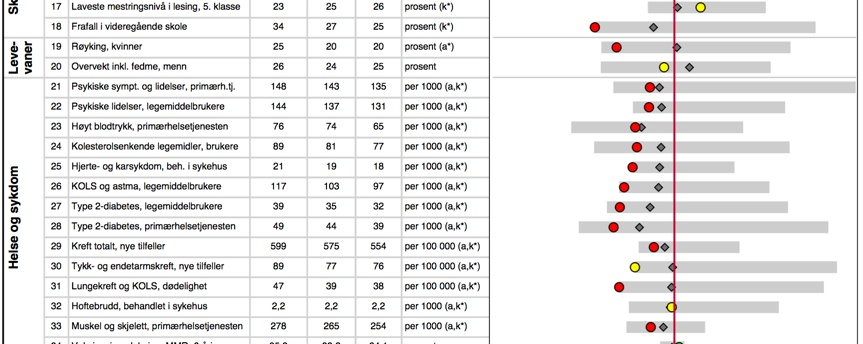
\includegraphics{./fhprofilnek.jpg}%placeholder
                      \caption[Utdrag fra folkehelseprofilen i Nedre Eiker]%\textit{tjenestetilbudene}.]
                      {Figuren viser et utdrag fra folkehelseprofilen i Nedre Eiker. Her er det mye å ta fatt i, men også enkelte lyspunkter.\cite{fhprofil}}
                    \end{figure}    

%Her slutter grafikken            

	\section{Eksisterende planverk}
	\section{Hvordan virkeligheten ser ut}

\chapter{Fokusområde: Fysisk helse}
	\section{Hvorfor fysisk helse?}
	\section{Hvordan måle effekten}
	\section{Suksessfaktorer}


\chapter{Gjennomføring}
	\section{Finansiering}
	\section{Administrative forutsetninger}
	\section{Første skritt på veien}

 \renewcommand{\bibname}{Kilder:}
              \begin{thebibliography}{99}

                \bibitem{Stmld47}
                  Helse- og Omsorgsdepartementet,
                  \emph{Stortingsmelding 47, 06/2009, Samhandlindlingsreformen}.
                  Hansen, Bjarne Haakon m. fl. (Minister)

                 \bibitem{fhprofil}
                  Folkehelseprofilen i Nedre Eiker
                  \emph{Folkehelseinstiuttet}.
                  

\end{thebibliography}


\end{document}